\documentclass[dvipdfmx]{jarticle}
\usepackage{graphicx}
\usepackage{url}
\usepackage[top=30truemm,bottom=30truemm,left=25truemm,right=25truemm]{geometry}
\usepackage{listings,jvlisting}

\lstset{
  basicstyle={\ttfamily},
  identifierstyle={\small},
  commentstyle={\smallitshape},
  keywordstyle={\small\bfseries},
  ndkeywordstyle={\small},
  stringstyle={\small\ttfamily},
  frame={tb},
  breaklines=true,
  columns=[l]{fullflexible},
  numbers=left,
  xrightmargin=0zw,
  xleftmargin=3zw,
  numberstyle={\scriptsize},
  stepnumber=1,
  numbersep=1zw,
  lineskip=-0.5ex
}

\begin{document}
\begin{titlepage}
    \begin{center}
        {\huge 情報科学演習C 課題3レポ―ト}
        \vspace{180pt}\\
        \begin{tabular}{rl}
            氏名 & 山久保孝亮\\
            所属 & 大阪大学基礎工学部情報科学科ソフトウェア科学コース\\
            メールアドレス & u327468b@ecs.osaka-u.ac.jp\\
            学籍番号 & 09B22084\\
            提出日 & \today\\
            担当教員 & 平井健士,中島悠太
        \end{tabular}
    \end{center}
\end{titlepage}
\section{課題3-1}
\subsection{アルゴリズム}
この課題の処理の流れは以下図1のフローチャートのとおりである.
\begin{figure}[h]
    \centering
    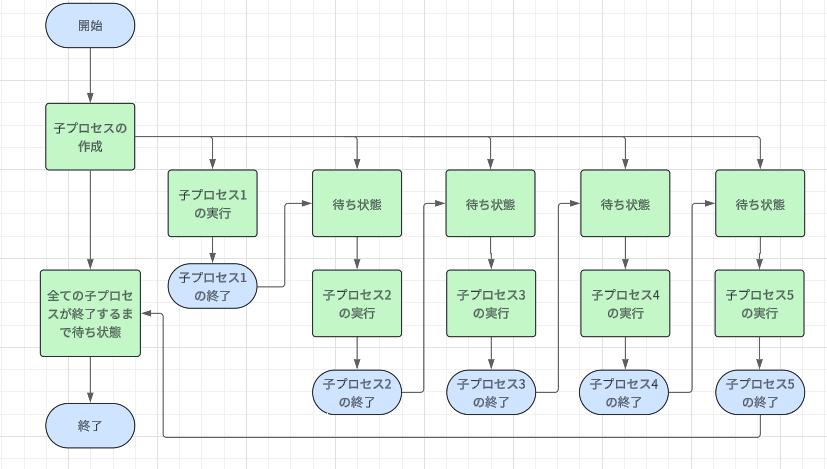
\includegraphics[width=12cm]{3-1hurotya.png}
    \caption{課題3-1の処理の流れ}
\end{figure}
\\
今回のfile-counterプログラムでは子プロセスを4つ作成し,それぞれの子プロセス内の処理を順番に一つずつ実行していく必要がある.
そのため,実行している子プロセス以外は待ち状態にしておき,実行が終了してから一つだけ待ち状態を開放して処理を実行するというアルゴリズムで今回の課題を実装した.フローチャートにおいて,子プロセスの終了から待ち状態へ伸びている矢印は
子プロセスが終わってから矢印の先の待ち状態が解放されるということを表している.今回の課題のクリティカルセクションは後述のcount1関数なので,この直前に待ち状態と解放を処理する関数を呼び出すようにした.
\subsection{実装方法}
ここではセマフォの処理について中心に記述する.以下は今回のプログラムにおける親プロセスの処理の流れである.
\begin{enumerate}
    \item セマフォセットの初期設定
    \item 子プロセスの作成
    \item 子プロセスがすべて終了するまで待つ
    \item セマフォの削除
\end{enumerate}
以下でその詳細について記述する.
\begin{enumerate}
    \item まず,ftok()を使ってkeyを作成する.このとき,第一引数の"."は現在のディレクトリを表し,第二引数の"1"はプロジェクトを一意に識別する文字を指定している.\cite{1}次にsemget()を使ってセマフォセットを作成している.
    第一引数は作成したkey,第二引数はセマフォの数である4,第三引数はアクセス許可の定義として使用され,全てに読み込み,書き込み許可を与えるという設定である.\cite{2}最後にsemctl()を使って0番目のセマフォの値を1に設定する.
    第一引数はセマフォIDのsem\_idを,第二引数でセマフォ番号の0を,第三引数のSETVALはsemvalの値を第四引数で指定された値に設定する制御操作を指定するパラメータ値である.セマフォの初期値を1に設定する理由については子プロセス
    にて詳細を記述する.
    \item fork()を使って子プロセスを作成する.for文の中で呼び出すことによって子プロセスを複数作成する.fork()の返り値をpidに格納し,pidの値によって子プロセスを分岐させて親プロセスと子プロセスの処理内容を分ける.
    ここでは親プロセスについて記述するので,その後の親プロセスの処理について記述する.
    \item wait()を使って子プロセスの終了を待つ.引数には状況の情報値を格納する.2で作成したプロセスの数だけfor文でこれを繰り返すことですべてのプロセスが終了するまで待ち続けることができるようになる.\cite{3}
    \item 最後にセマフォをsemctl()を使って削除する.第三引数のIPC\_RMIDは第一引数によって指定されたセマフォIDをシステムから除去し,それに関連するセマフォセットを破棄する.\cite{2}
\end{enumerate}
また,子プロセスのプログラムは以下のようになる.
\begin{lstlisting}
if (pid == 0) { /* Child process */
    lock(sem_id);
    count = count1();
    printf("count = %d\n", count);
    unlock(sem_id);
    exit(0);
}
\end{lstlisting}
以下でその詳細について記述する.
\begin{enumerate}
    \item 2においてpidの値が0のときは子プロセスであると判定できる.子プロセス内の処理がクリティカルセクションであるので,まずlock()を呼び出す.lock()では,semop()を使ってプロセスを停止している.第一引数はセマフォIDのsemid
    ,第二引数はsembuf構造体のポインタ,第三引数は第二引数の数を表す.sembuf構造体は3津のメンバが存在し,sem\_numはセマフォ番号,sem\_opはセマフォ操作,sem\_flagは操作フラグを表す.\cite{4}sem\_opは-1,それ以外は0に指定することによって
    セマフォ値がsem\_opの値を足した結果0以上にならない場合はプロセスを停止する.セマフォ値の初期値を1にしていたことによって,最初のプロセスは停止しないが,次のプロセスはセマフォ値が0でsem\_opを加算すると負の値になってしまうので
    停止する.
    \item セマフォに関係する処理はないので省略する.
    \item unlock()ではsemop()を使ってセマフォ値を変更し,子プロセスの待ち状態を一つ開放する.第二引数のsembuf構造体のsem\_opを1に,それ以外を0に設定することによって待っている一つの状態の子プロセスにおいて
    -1を加算してもセマフォ値が0以上になるので待ち状態ではなくなる.このようにして待ち状態のプロセスの開放を一つずつ行うことによってbクリティカルセクションに複数のプロセスが同時にアクセスできないようにしている.
    \item exit()を使って子プロセスを終了する.
\end{enumerate}
\subsection{実行結果}
この実行結果は以下のようになる.  \clearpage
\begin{figure}[htbp]
    \begin{minipage}[b]{0.45\linewidth}
      \centering
      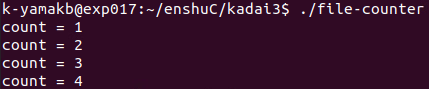
\includegraphics[keepaspectratio, scale=0.7]{result3-1.png}
      \caption{ターミナル上の実行結果}
    \end{minipage}
    \begin{minipage}[b]{0.45\linewidth}
      \centering
      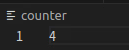
\includegraphics[keepaspectratio, scale=0.8]{result3-1-1.png}
      \caption{counterファイルの内容}
    \end{minipage}
  \end{figure}
  以上の結果により,きちんとcountが1ずつ増やされ,最終的にcounterファイルには4が記入されているということがわかる.
\section{課題3-2-1}
\subsection{アルゴリズム}
この課題の処理の流れは以下図3のフローチャートのとおりである.
\begin{figure}[h]
    \centering
    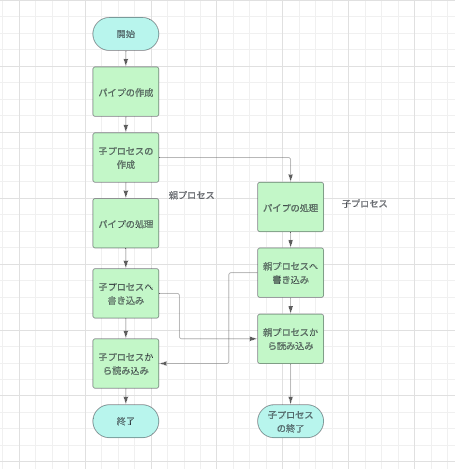
\includegraphics[width=8cm]{3-2hurotya.png}
    \caption{課題3-2の処理の流れ}
\end{figure}
\\
今回のtwo-way-pipeプログラムでは子プロセスを一つ作成し,子プロセスから親プロセスへ最初の引数の文字列を,親プロセスから子プロセスへ次の引数の文字列を送信する.
そして親プロセスは子プロセスから,子プロセスは親プロセスから送られてきた文字列を受け取り標準入力に表示させる.図の左側は親プロセス,右側は子プロセスの処理を表す.
双方向のパイプを実現するために,子プロセス用のパイプと親プロセス用のパイプの二つのパイプを作成して実装した.これは,パイプは安全のために書き込み側か読み込み側のどちらかをっクローズする必要があるため,
一つのパイプではどちらの機能も同時に使うことができないためである.
\subsection{実装方法}
パイプ部分を中心に実装方法を記述する.
\begin{enumerate}
    \item パイプの作成は,pipe()を使って行う.親プロセスから子プロセスへ送信したり,親プロセスが読み込むためのパイプとしてparenttochild,子プロセスから親プロセスへ送信したり,子プロセスが読み込むためのパイプとしてchildtoparent
    を定義した.
    \item fork()を使って子プロセスを一つ作成し,pidが0かどうかで親プロセスと子プロセスの処理を分離した.子プロセスではparenttochildの書き込み機能とchildtoparentの読み込み機能を使用しないので,これらをclose()しておく.
    そして第二引数の文字列をwrite()を使って送信しread()を使って親プロセスから送られてきた第一引数の文字列を受信して標準出力に出力する.また,親プロセスではparenttochildの読み込み機能とchildtoparentの書き込み機能を使用しないのでこれらをclose()しておく.
    そして第一引数の文字列をwrite()を使って送信しread()を使って子プロセスから送られてきた第二引数の文字列を受信して標準出力に出力する.
\end{enumerate}
\subsection{実行結果}
\section{課題3-2-2}
\subsection{アルゴリズム}
この課題の処理の流れは以下図5のフローチャートのとおりである.
\begin{figure}[h]
    \centering
    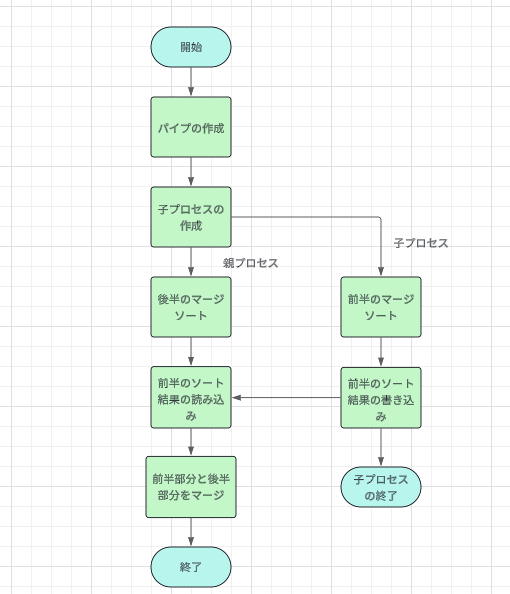
\includegraphics[width=8cm]{3-2-2hurotya.png}
    \caption{課題3-2の処理の流れ}
\end{figure}
\\
今回のmergesortプログラムでは子プロセスを一つ作成し,子プロセスでソート対象の配列の前半半分を,親プロセスでソート対象の配列の後半半分をソートしてからマージするというアルゴリズムで作成した.
図5の左側が親プロセス,右側が子プロセスに対応する.また,子プロセスのソート結果を親プロセスに伝えるためにパイプを使用した.これにより前半と後半のソートを並列に実行できるようになる.
\subsection{実装方法}
ここではマージソートのアルゴリズムについては言及せず,どのようにして並列化をしたかについて中心に記述する.関数mergesort中に図5のフローチャートの流れで並列化を実装したのでそれぞれの詳細について記述する.
\begin{enumerate}
    \item pipe()を使ってパイプfdを作成した.
    \item fork()を使って子プロセスを作成し,pidが0かどうかで親プロセスと子プロセスの処理を分離した.子プロセスではfdの読み込み機能は使用しないのでclose()しておく.引数には0と配列の要素の中央値を渡してmsort()呼び出す.
    これによってソート対象の配列の前半部分をマージソートすることができる.次にwrite()を呼び出して前半がソートされた配列を親プロセスに送信する.このときに引数に0と配列の要素の中央値を渡すことで配列全体ではなく前半部分のみを送ることができる.
    配列全体を送ってしまうと親プロセスでソートされた部分と競合してしまい,正しいソート結果ではなくなってしまう.
    \item 親プロセスではfdの書き込み機能は使用しないのでclose()しておく.親プロセスでは引数として配列の要素数の中央値と配列の要素数を渡してmsort()を呼び出す.これによってソート対象の配列の後半部分をマージソートすることができる.
    その後read()を使って子プロセスから送信された前半のソート結果を読み込む.このときに引数に配列の0と配列の要素数の中央値を渡すことで前半部分だけを読み込む.
    \item 最後に前半部分と後半部分をmergesort()を呼び出してソートする.
\end{enumerate}
\subsection{実行結果}
\section{課題3-3-1}
\subsection{アルゴリズム}
この課題の処理の流れは以下図のフローチャートの通りである.
\begin{figure}[h]
    \centering
    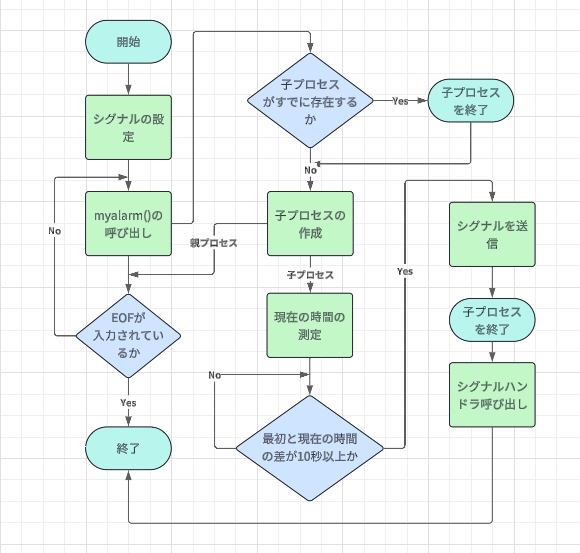
\includegraphics[width=8cm]{3-3-1.png}
    \caption{課題3-3-1の処理の流れ}
\end{figure}
\\
今回の課題ではalarmプログラム内のmyalarm()をalarm()を使用せずに実現するというものである.alarm()は子プロセスが引数で指定した秒数secだけ経つとシグナルを送信し,親プロセス内でシグナルハンドラが呼び出される.
上図フローチャートの左部がmain()の処理,中央と右部がalarm()の処理を表している.
\subsection{実装方法}
今回の課題ではmyalarm()内の実装のみを求められているので,myalarm()の実装方法について詳細に記述する.
fork()の返り値をタイマー管理用のプロセスIDを格納しているグローバル変数timer\_pidに格納している.この変数は最初に-1に初期化されているので,myalarm()の呼び出しが初めてなのかどうかを子の変数の値によって判定することができる.
まず最初にtime\_pidが正であるかどうかを判定している.fork()の返り値はなので,正であれば初めてのmyalarm()の呼び出しではないので,前回作成した子プロセスを終了させ,waitpid()を使って子プロセスの終了を待つことでゾンビプロセスが発生することを避ける.
次に時間経過を測定するためにfork()を使用して子プロセスを作成し,pidによって条件分岐することで親プロセスと子プロセスの処理を分ける.
親プロセスでは前述の通りtimer\_pidにfork()の返り値を格納する.子プロセスではwhile文の繰り返しを一定時間が経過するまで繰り返し続けることで一定時間の計測を実現している.
具体的には,myalarm()を呼び出したときの時刻とwhile文のそれぞれの繰り返し時の時刻との差を格納しているelapsed\_secondsと指定したsecを比較し,前者の方が大きくなった際にループを抜けるという処理としている.
自刻の計測にはtime()を使用し,差の計算にはdifftime()を使用した.そしてループを抜けた後にkill()を使ってシグナルハンドラを起動するシグナルを送り,子プロセスを終了する.
\subsection{実行結果}
\section{課題3-3-2}
\subsection{アルゴリズム}
この課題の処理の流れは以下のフローチャートの通りである.
\begin{figure}[h]
    \centering
    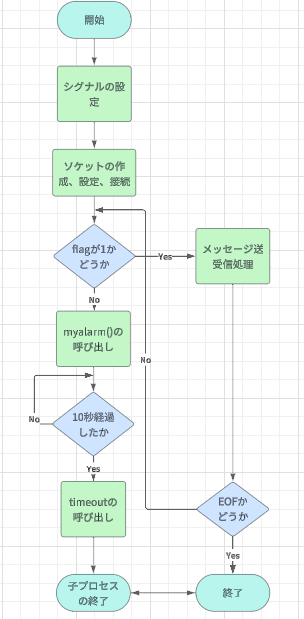
\includegraphics[width=7cm]{3-3-2.png}
    \caption{課題3-3-2の処理の流れ}
\end{figure}
\\この課題は大部分が課題2の内容なので,以下では追加した点について中心に記述する.図5のmyalart()の呼び出しの下側は子プロセスの処理,右側は親プロセスの処理となっている.
また,それぞれのプロセスの終了から出ている両方向への有向辺は一方のプロセスが終了するともう一方のプロセスの処理も終了するということを示している.
これによって,10秒間経過するかEOFが入力されたときにどちらのプロセスも終了させることができる.
\subsection{実装方法}
以下では4で述べたmyalarm()を使用するので,この関数については詳細を記述しない.
今回の課題に当たって変更した点は以下の5つである.
\begin{enumerate}
    \item シグナル送信の設定
    \item myalarm()の呼び出し
    \item シグナルハンドラtimeoutの設定
    \item タイムアウトの条件分岐
    \item while分の繰り返し条件の変更
\end{enumerate}
以下でその詳細について述べる.
\begin{enumerate}
    \item シグナル送信の設定は課題3-5-1と同様に設定した.
    \item myalarmの呼び出しは,selectによる待ち状態になる前,即ちサーバと接続されたときまたは標準入力へEOF以外の書き込み
    が起こったときに行われる.alarm()は一度呼び出されてから10秒以内にもう一度呼び出すと前回呼び出した際のプロセスを終了する.これによって,何も入力されない状態が10秒続けば
    シグナルが送信されプログラムが終了するという機能が達成される.
    \item シグナルハンドラは仕様により非同期安全な関数のみしか使用できない.したがって,printfのような関数は使用できないため,今回のプログラムではシグナルハンドラtimeout内では
    flagという変数の値を変更するだけとした.このflagは子プロセス内で10秒が経過したときに1となり,それ以外は0のグローバル変数である.
    \item タイムアウトが発生すると先ほどシグナルハンドラで立てたflagが1となる.その条件分岐をselect()による待ち状態の直前,即ちmyalarm()の後に配置すると10秒経った時点で
    if分の内部の式が実行される.そこではソケットを閉じて,タイムアウトが発生したと標準出力に表示してからexit()によってプログラムを終了する.
    \item 課題2のsimple-talk-clientではメッセージ送受信を複数回行うためのwhile文の繰り返し条件は1で,無限ループだったが,今回の課題ではその条件式をflagが1出ない限り繰り返すという条件に変更した.
    これによって,10秒以内にメッセージを送受信し続ける限り,flagが立たないので無限に繰り返し続けることができるようになる.
\end{enumerate}
\subsection{実行結果}
\section{発展課題1}
\subsection{アルゴリズム}

\subsection{実装方法}

\subsection{実行結果}

\section{発展課題2}
\subsection{アルゴリズム}
今回の課題では課題3-2-2における,子プロセスによるマージソートを高速化プログラムを改良し,指定された任意のk個のプロセスに
配列を分解してソートするプログラムを作成した.
この課題ではmergesort()の部分のみを変更したのでその部分のフローチャートを以下に示す.
\begin{figure}[h]
    \centering
    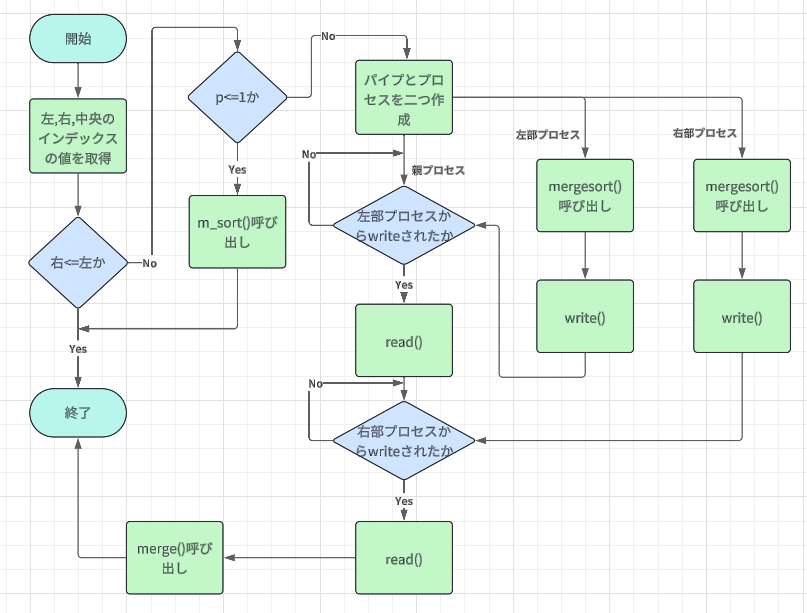
\includegraphics[width=8cm]{hatten2hurotya.png}
    \caption{mergesort()のフローチャート}
\end{figure}
フローチャート中のpは,そのプロセスにおいて作成しなければならないプロセスの個数を表す.\\
このプログラムでは任意のk個のプロセスに分解する方法として二分木の形状で再帰的にmergesort()を呼び出すという方法を採用した.具体的には,以下の手順に従っている.
\begin{enumerate}
    \item 配列を右部と左部に分け,それぞれに対応する子プロセスを作成する.以下ではこれらをそれぞれ左部のプロセス1.1と右部のプロセス1.2と呼ぶ.各プロセスの数字は二分木におけるの深さと左から何番目であるかに対応するものとする.
    このとき,子プロセスを作成してmergesort()を呼び出すがその際のpは左部のプロセスでは$p_left=\frac{p}{2}$,右部のプロセスでは$p_right=p-p_left$として引数にする.
    \item さらにプロセス1.1を左部のプロセス2.1と右部のプロセス2.2に分ける.右プロセスも同様に分ける.
    \item 合計の子プロセスの個数が指定したkに達するまで行う.kに達したかどうかは引数として与えているpの値が子プロセスになるにつれて減少していることから判断する.
\end{enumerate}
実際に9個のプロセスに分けると考えたときの二分木の様子は以下のようになる.
\begin{figure}[h]
    \centering
    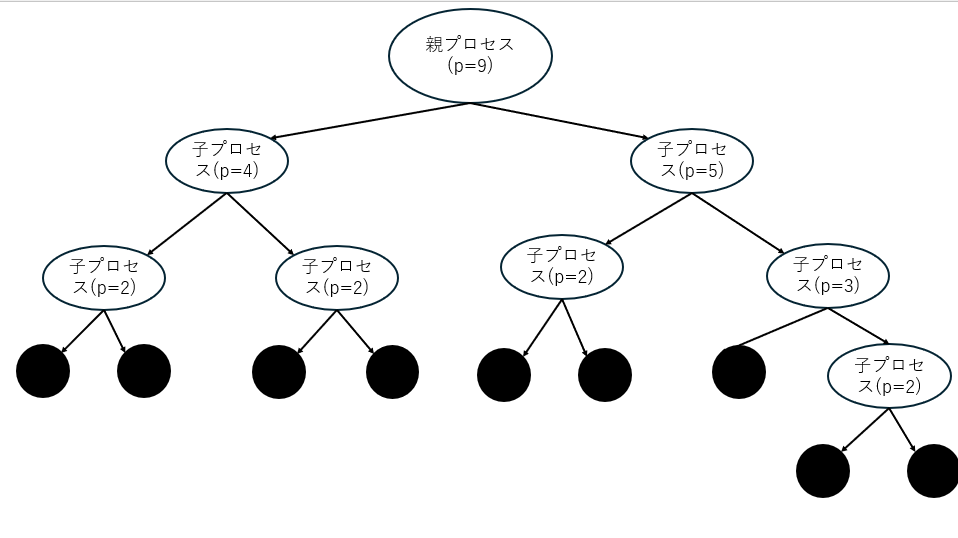
\includegraphics[width=8cm]{hatten2tree.png}
    \caption{実際にプロセスに分ける様子}
\end{figure}
黒い葉はp=1のときの子プロセスを表しており,それぞれの白い節点で葉の処理が終わってからmerge()が呼び出される.

\subsection{実装方法}
mergesort()の引数は以下のようになっている.
\begin{lstlisting}
    void mergeSort(int numbers[], int temp[], int left, int right, int p);
\end{lstlisting}
numbersとtempは課題3-2-2と同じで,ソートする対象の左端と右端を表すleftとright,そのプロセスにおいて作成しなければならないプロセスの個数であるpを引数として追加した.
先ほどのアルゴリズムで示したように,mergesort()を再帰的に呼び出す処理を行う.そのための処理としては以下のプログラムのようになる.
\begin{lstlisting}
if (left_pid == 0) {
    close(fd_left[0]);
    mergeSort(numbers, temp, left, mid, p_left);
    if (write(fd_left[1], &numbers[left], size_left * sizeof(int)) == -1) {
        perror("pipe write.");
        exit(1);
    }
    close(fd_left[1]);
    exit(0);
}
\end{lstlisting}
上は左部プロセスについての処理である.再帰的に呼び出すために,mergesort()の引数として左端をleft,右端を$mid = \frac{left+right}{2}$とした.
\begin{lstlisting}
if (right_pid == 0) {
    close(fd_right[0]);
    mergeSort(numbers, temp, mid + 1, right, p_right);
    if (write(fd_right[1], &numbers[mid + 1], size_right * sizeof(int)) == -1) {
        perror("pipe write.");
        exit(1);
    }
    close(fd_right[1]);
    exit(0);
}
\end{lstlisting}
また,右部プロセスについての処理である.再帰的に呼び出すために,mergesort()の引数として左端をmid+1,右端をrightとした.パイプの処理についてはどちらのプロセスでも書き込みをしたいので二つのパイプfd\_leftとfd\_right
を使用した.そして左部プロセスと右部プロセスの両方が終了すればそのプロセスにおけるleft,mid,rightを使ってmerge()を実行する.
\subsection{実行結果}
\section{発展課題3}
\subsection{アルゴリズム}
ここでは交互実行をセマフォを使って実装した.具体的な処理の流れは以下のフローチャートのようになる.
\begin{figure}[h]
    \centering
    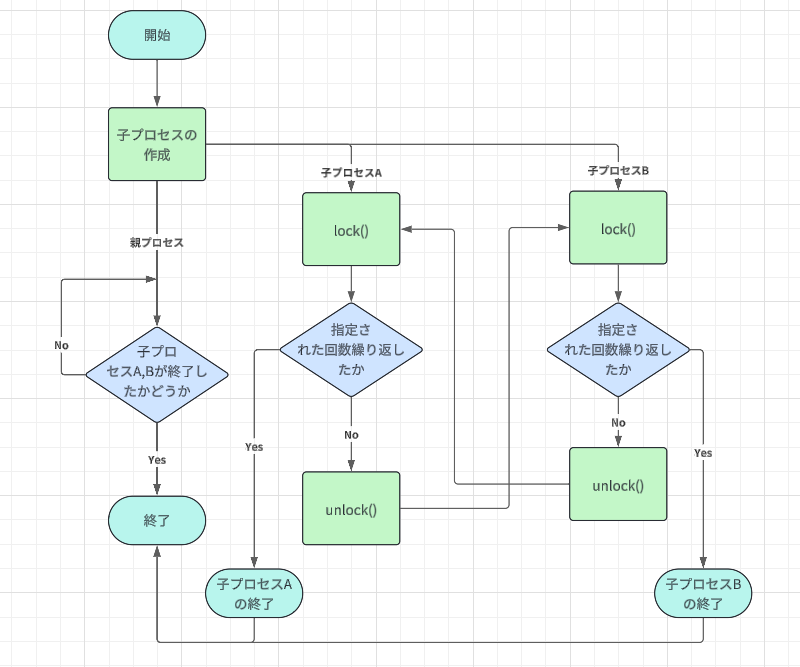
\includegraphics[width=8cm]{hatten3hurotya.png}
    \caption{発展課題3のフローチャート}
\end{figure}
\\ここで登場するlock()とunlock()は課題3-1で使用したものと同じである.unlock()からlock()に有向辺が出ているのは,セマフォの値をunlock()で増加させることで,lock()により待ち状態であったもう一方の子プロセスを開放するということを表す.
これにより,お互いに待ち状態と実行状態を交互に繰り返すようにした.
\subsection{実装方法}
実装方法としては,以下のとおりである.
\begin{enumerate}
    \item セマフォ用のキーを作成し,セマフォセットを作成して初期値を1とする.
    \item 子プロセスを二つ作成する.子プロセスAではグローバル変数の配列A\_listを要素数だけ標準出力に出力する.子プロセスBではグローバル変数の配列B\_listを要素数だけ標準出力に出力する.
    \item 親プロセスでは子プロセスの終了を待ち,両方のプロセスが終了すればセマフォを開放する.
\end{enumerate}
いかに詳細を記述する.
\begin{enumerate}
    \item ここは課題3-1と同様なので省略する.
    \item 子プロセスAの処理は以下のようなプログラムである.
    \begin{lstlisting}
        if (a_pid == 0) { // 子プロセスA
        for (int i = 0; i < NUM; i++) {
            lock(sem_id);
            printf("a%d\n", A_list[i]);
            unlock(sem_id);
        }
        exit(0);
    }
    \end{lstlisting}
    NUMには配列A\_listとB\_listの要素数を表す変数が格納されており,printf()が呼ばれるたびにlock()とunlock()が上のようなタイミングで呼び出される.
    これは課題3-1の時と同様にセマフォの値がunlock()を呼び出すたびに1増加されてもう一方のプロセスで待ち状態が解放されて処理が始まるということを表し,これにより交互に実行することが実現される.
    \\
    また,子プロセスBの処理は以下のようなプログラムである.
    \begin{lstlisting}
        if (b_pid == 0) { // 子プロセスB
        for (int i = 0; i < NUM; i++) {
            lock(sem_id);
            printf("b%d\n", B_list[i]);
            unlock(sem_id);
        }
        exit(0);
    }
    \end{lstlisting}
    これも子プロセスAと同様である.
    \item プロセスの待ちとセマフォの開放は以下のようになる.
    \begin{lstlisting}
    wait(NULL);
    wait(NULL);

    // セマフォを解放
    if (semctl(sem_id, 0, IPC_RMID) == -1) {
        perror("semctl IPC_RMID エラー.");
        exit(1);
    }
    \end{lstlisting}
\end{enumerate}
\subsection{実行結果}

\section{考察}
今回の課題を通して私が考察したのは,
\begin{thebibliography}{99}
    \bibitem{1} \url{https://www.ibm.com/docs/ja/aix/7.3?topic=f-ftok-subroutine} 6/12アクセス
    \bibitem{2} \url{https://www.ibm.com/docs/ja/aix/7.3?topic=s-semget-subroutine} 6/12アクセス
    \bibitem{3} \url{https://www.ibm.com/docs/ja/zos/2.5.0?topic=functions-wait-wait-child-process-end} 6/12アクセス
    \bibitem{4} \url{https://www.c-lang.net/semop/index.html} 6/12アクセス
\end{thebibliography}
\end{document}